\documentclass[final]{beamer}
  \mode<presentation> {\usetheme{I6pd2}}
  \usepackage{type1cm}
  \usepackage{calc} 
  \usepackage{times}
  \usepackage{amsmath,amsthm, amssymb, latexsym}
  \usepackage{adjustbox}
  \boldmath

  \usepackage{tikz}
  \usetikzlibrary{shapes,arrows,decorations.text}

  \usepackage[english]{babel}
  \usepackage[latin1]{inputenc}
  \usepackage[orientation=portrait,size=a0,scale=1.4,grid,debug]{beamerposter}

  \title[BESDIRAC Transfer System]{\Huge Dataset-based High-Level Data Transfer
  System in BESDIRAC}
  \author[Tao \& Xiaomei]{Tao Lin and Xiaomei Zhang}
  \institute{Institute of High Energy Physics}
  \date{Oct. 14th-18th, 2013}

% Create a counter
\newcounter{blockcounter}
\setcounter{blockcounter}{0}

\newenvironment{myblock}[1]{
    \vfill
    \begin{block}{\stepcounter{blockcounter}\arabic{blockcounter} #1}
} {
    \end{block}
    \vfill
}

\begin{document}

\begin{frame}{}
    
% Abstract    
\begin{columns}[c]

    \begin{column}{.95\textwidth}
    \begin{beamercolorbox}[wd=\textwidth]{postercolumn}
\begin{block}{Abstract}
Data Transfer is an essential part in grid.
In the BESIII experiment, the result of Monte Carlo Simulation should 
be transfered back from other sites to IHEP and the DST files for physics analysis 
should be tranfered from IHEP to other sites. A robust transfer system should 
make sure all data are transfered correctly.
In this poster, the design and implementation of a 
Dataset-based Data Transfer System will be shown.

\end{block}
    \end{beamercolorbox}
    \end{column}
\end{columns}

% Content

    \begin{columns}[c]
        \begin{column}{.01\textwidth}
        \end{column}
        % --------------------------------------------------------------------
        % column 1
        \begin{column}{.48\textwidth}
            \begin{beamercolorbox}[center,wd=\textwidth]{postercolumn}
                
\begin{myblock}{BESIII experiment}
    \begin{itemize}
        \item BESIII experiment is a general purpose experiment
              for studying electron-positron collisions at BEPCII.
        %\item Since spring 2009, large scale raw data has produced.
        \item The BESIII data production uses both 
              a local cluster model and a distributed computing model.
        \item DIRAC is a solution for the distributed computing.
    \end{itemize}
\end{myblock}

\begin{myblock}{Why need a dataset-based Transfer System?}
    \begin{itemize}
        %\item The result of Monte Carlo Simulation (or Reconstruction)
        %      should be transfered back from other sites to IHEP.
        %\item The files for physics analysis should be transfered
        %      from IHEP to others sites.
        \item The result of Monte Carlo Simulation
        \item The files for physics analysis
        \item If there is a transfer system:
            \begin{itemize}
                \item the user don't need to wait and monitor the status;
                \item user can retransfer failed files easily.
                %\item the administrator can monitor the status of the sites
                %      and analysis these status.
            \end{itemize}
    \end{itemize}
\end{myblock}

\begin{myblock}{Developing in DIRAC \& BESDIRAC}
    \begin{itemize}
        %\item The DIRAC (Distributed Infrastructure with Remote Agent Control)
        %      project is a complete Grid solution for a community of users
        %      needing access to distributed computing resources. 
        %      {\em from diracgrid.org}
        \item DIRAC consists of cooperation distributed {\em services}
              and light-weight {\em agents} delivering the workload to 
              the Grid Resources.
        \item We can {\em reuse} the most functionalities supplied by DIRAC.
        \item BESDIRAC is an extension to DIRAC for BESIII specified.
    \end{itemize}
\end{myblock}

\begin{myblock}{DIRAC Architecture}
    \begin{columns}
        \column{.6\linewidth}
            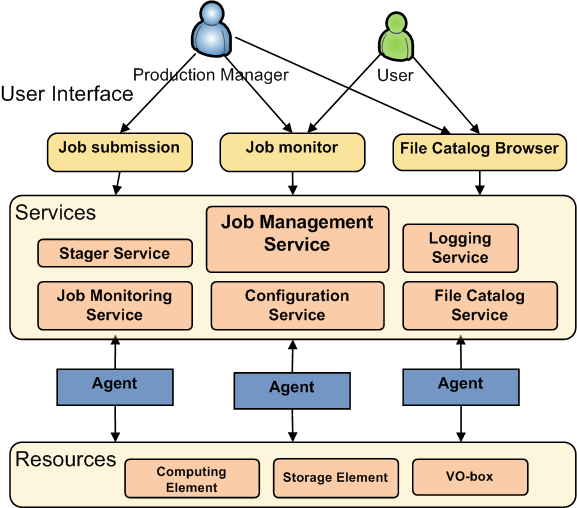
\includegraphics[width=\textwidth,keepaspectratio]{figures/DIRAC_Architecture.png}
        \column{.4\linewidth}
            DIRAC follows the {\tt Service Oriented Architecture (SOA)}
            paradigm, accompanied by a network of lightweight distribued
            agents which animate the system.
            
            \begin{itemize}
                \item User Interfaces
                \item Services
                \item Agents
                \item Resources
            \end{itemize}
    \end{columns}
\end{myblock}

\begin{myblock}{Members in Transfer System}
    \begin{itemize}
        \item In the transfer system, we have:
        \begin{description}
            \item[Transfer Agent] is the scheduler to create the transfer
                 processes.
            \item[Tranfer Request Service] is to create, kill, retransfer
                 and monitor the transfer requests.
            \item[Dataset Service] is to create and show the dataset.
        \end{description}
        \item In Dirac File Catalog, dataset is dynamic.
        \item Dataset Service is a temporary solution for the static
              dataset.
    \end{itemize}
\end{myblock}

\begin{myblock}{The workflow of Transfer System}
    % Define block styles
\begin{center}
\tikzstyle{block} = [rectangle, draw, fill=blue!20, text width=4em, text centered, rounded corners]
\tikzstyle{hugeBlock} = [rectangle, draw, fill=blue!20,
    text width=5em, text centered, rounded corners, minimum height=3em]
\tikzstyle{line} = [draw, -latex, line width=.1em]

%\adjustbox{max width=\textwidth}{
\begin{tikzpicture}[node distance = 2cm, auto]
    \node [block] (user) {User};
    \node [block, right of=user, node distance=4cm] (transReqSvc) {Transfer Request Service};
    \node [block, below of=user, node distance=1.4cm] (DFC) {DFC};
    \node [block, right of=DFC, node distance=4cm] (datasetSvc) {Dataset Service};
    \node [block, right of=transReqSvc, node distance=4cm, yshift=-0.7cm, 
            text width=6em]
                                                    (Database) {TransferDB};
    \node [block, right of=Database, node distance=4cm] (transAgent) { Transfer Agent};
    \path[line,<->, postaction={
                    decorate,
                    decoration={
                        raise=1ex,
                        text along path,
                        text align=center,
                        text={2},
                    }
        }](user) -- (transReqSvc);
    \path[line,->, postaction={
                    decorate,
                    decoration={
                        raise=1ex,
                        text along path,
                        text align=center,
                        text={1},
                    }
        }] (user) -- (DFC);
    \path[line,->](DFC) -- (datasetSvc);
    \path[line,<->](transReqSvc) -- (Database);
    \path[line,<->](datasetSvc) -- (Database);
    \path[line,<->,postaction={
                    decorate,
                    decoration={
                        raise=1ex,
                        text along path,
                        text align=center,
                        text={3},
                    }
        }](Database) -- (transAgent);
\end{tikzpicture}
%} % adjustbox
\end{center}

    \begin{enumerate}
        \item User create a snapshot of the file list in DFC, 
              which is registered in the Dataset Service.
        \item User create or modify or monitor the transfer request.
        \item Transfer Agent will transfer these files in the Database.
    \end{enumerate}
\end{myblock}

            \end{beamercolorbox}
        \end{column}
        % --------------------------------------------------------------------
        \begin{column}{.01\textwidth}
        \end{column}
        % --------------------------------------------------------------------
        % column 2
        \begin{column}{.48\textwidth}
            \begin{beamercolorbox}[center,wd=\textwidth]{postercolumn}


%\begin{myblock}{TransferDB}
%    \begin{center}

    \tikzstyle{mytable} = [rectangle, draw, text centered,
        %rectangle split, rectangle split parts=2
    ]
    \tikzstyle{line} = [draw, -latex, line width=.1em]

\begin{tikzpicture}
    \node[mytable](transreq) {
        \begin{tabular}{l}
        \textbf{Transfer Request}
        \\
        \hline
        id \\
        username \\
        dataset \\
        srcSE \\
        dstSE \\
        protocol \\
        submit\_time \\
        status \\
        \end{tabular}
    };
    \node[mytable, right of=transreq, node distance=15cm](transfilelist) {
        \begin{tabular}{l}
        \textbf{Transfer File List}
        \\
        \hline
        id \\
        LFN \\
        trans\_req\_id \\
        start\_time \\
        finish\_time \\
        status \\
        error
        \end{tabular}

    };
    \path[line,-] (transreq.east)++(0,4.5) -- ++(2, 0.0) 
                            |- ++(2,-3.9)

              ;
\end{tikzpicture}

\end{center}

%\end{myblock}

\begin{myblock}{Transfer Agent}
    \begin{itemize}
        \item In {\tt DIRAC}, {\tt AgentModule} is the base class for all {\tt
            Agent}s. The derived classes should implement:
        \begin{itemize}
            \item {\tt initialize}
            \item {\tt execute}
            \item {\tt finalize}
        \end{itemize}
        \item {\tt TransferAgent} implements the {\tt non-blocking}
              scheduler in the {\tt execute} method.
        \item In fact, we create several {\tt sub processes} to run the 
                transfer commands. The scheduler uses the {\tt async I/O}
                to communicate with the {\tt sub processes}.
        %\item To test more easily, we create a standard module {\tt helper}.
        %      It just uses the {\tt TransferDB} and some basic services supplied
        %      by {\tt DIRAC}, such as the {\tt Configuration Service}.
        %      So, we don't need to restart our agent to test the program.
        \item To support multiple transfer protocols, we use a {\tt
                TransferFactory} to create {\tt TransferWorker}s.
    \end{itemize}
\end{myblock}

\begin{myblock}{The workflow of Transfer Agent}
    \begin{center}
\tikzstyle{decision} = [diamond, draw, fill=blue!20, 
                        text width=4.5em, text centered, 
                        node distance=3cm, inner sep=0pt]
\tikzstyle{block} = [rectangle, draw, fill=blue!20, text width=4em, text centered, rounded corners]
\tikzstyle{line} = [draw, -latex, line width=.3em]

\pgfdeclarelayer{background}
\pgfdeclarelayer{foreground}
\pgfsetlayers{background,main,foreground}

\begin{tikzpicture}[node distance = 2cm, auto]

    % The Main Loop contains
    % * check existing work node
    % * add new transfer

    % PART I 
        \node [block] 
            (part1) {check existing worker};
    % PART II
        \node [block, below of=part1, node distance =10.5cm] 
            (part2) {add new worker};

    % LINE part1 -> part2
        \path[line,->]
            (part1) -- (part2);
    % LINE part2 -> part1
        \path[line,->]
            (part2.south) |- ++(-5.5,-0.8)
            -- ++(0, 16.5)
            -| (part1.north);

    % in PART I
    % * check status of the worker in DB
        \node [block, right of=part1, node distance=8cm]
            (statusInDB) {check worker status in DB};
    % * check terminate or not
        \node [decision, right of=statusInDB, node distance=7cm]
            (terminateOrNot) {Termiated?};
    % * NO
    %   + dump info
    % * Yes
    %   + remove worker from queue
        \node [block, right of=terminateOrNot, node distance=7cm]
            (rmInQueue) {Remove worker in the Queue};
    %   + handle exit code
        \node [block, right of=rmInQueue, node distance=7cm]
            (exitCode) {Handle exit code};
    %   + update status
        \node [block, below of=exitCode, node distance=6cm]
            (updateStatus) {Update DB};
    % * dummy object
        \node [below of=terminateOrNot, node distance=6cm]
            (dummyObj){};

    % LINE
    % * part1 -> statusInDB
        \path[line,->]
            (part1) -- (statusInDB);
    % * statusInDB -> terminateOrNot
        \path[line,->]
            (statusInDB) -- (terminateOrNot);
    % * terminateOrNot -> dummyObj
        \path[line,-]
            (terminateOrNot.south) -- node{No}(dummyObj.center);
    % * updateStatus -> dummyObj
        \path[line,-]
            (updateStatus.west) -- (dummyObj.center);
    % * terminateOrNot -> rmInQueue
        \path[line,->]
            (terminateOrNot) -- node{Yes}(rmInQueue);
    % * rmInQueue -> exitCode
        \path[line,->]
            (rmInQueue) -- (exitCode);
    % * exitCode -> updateStatus
        \path[line,->]
            (exitCode) -- (updateStatus);

    % * dummy object 
        \path[line,<-]
             (part1.east)+(0,-1) 
             -| ++(1,-6)
             -- node{RETURN} (dummyObj.center);

    % PART I Layer background
        \begin{pgfonlayer}{background}
            \path (statusInDB.north west)+(-0.5,0.5) node (g) {};
            %\path (bw.east |- syscomb.south)+(0.5,-1.5) node (h) {};
            \path (updateStatus.south east)+(0.5,-0.5) node (h) {};

            \path[fill=yellow!20,rounded corners,
            draw=black!50, dashed]
            (g) rectangle (h);
        \end{pgfonlayer}

    % in PART II
    % * IDLE
        \node [decision, right of=part2, node distance=8cm, aspect=2,
               inner sep=-5pt]
            (idle) {Idle?};
    % * Has New Request
        \node [decision, right of=idle, node distance=10cm, aspect=2,
               text width=5em, inner sep=-5pt]
            (newreq) {any reqs?};
    % * create worker
        \node [block, right of=newreq, node distance=10cm]
        (createworker) {create worker};

    % * dummy obj
        \node [below of=idle, node distance=3cm]
            (dummyObj2) {};
        \node [below of=newreq, node distance=3cm]
            (dummyObj3) {};

    % LINE
    % * part2 -> idle
        \path[line,->]
            (part2) -- (idle);
    % * idle -> newreq
        \path[line,->]
            (idle) -- node{Yes}(newreq);
    % * newreq -> createworker
        \path[line,->]
            (newreq) -- node{Yes}(createworker);
    % * idle -> dummy
        \path[line,-]
            (idle) -- node{No}(dummyObj2.center);
    % * newreq -> dummy
        \path[line,-]
            (newreq) -- node{No}(dummyObj3.center);
    % * createworker -> dummy
        \path[line,-]
            (createworker) |- (dummyObj2.center);
    % * dummy -> part2
        \path[line,<-]
            (part2.east)+(0,-1)
            -| ++ (1, -3)
            -- (dummyObj2.center);

    % PART II Layer background
        \begin{pgfonlayer}{background}
            \path (idle.north west)+(-1.8,1.3) node (g) {};
            %\path (bw.east |- syscomb.south)+(0.5,-1.5) node (h) {};
            \path (createworker.south east)+(0.5,-1.8) node (h) {};

            \path[fill=yellow!20,rounded corners,
            draw=black!50, dashed]
            (g) rectangle (h);
        \end{pgfonlayer}

\end{tikzpicture}
\end{center}

\end{myblock}

\begin{myblock}{Transfer Factory}
    
\begin{center}
    \tikzstyle{myclass} = [rectangle, draw, text centered]
    \tikzstyle{line} = [draw, -latex, line width=.1em]

\begin{tikzpicture}[scale=0.9]
    \node[myclass](ITransferWorker){ITransferWorker};
    \node[below of=ITransferWorker, node distance=3cm](DummyWorker){};
    \node[myclass,left of=DummyWorker, node distance=6cm]
            (DIRACDMSTW){DMSTransferWorker};
    \node[myclass,right of=DummyWorker, node distance=6cm]
            (DIRACFTSTW){FTSTransferWorker};
    \node[below of=DummyWorker, node distance=4cm](DummyWorker2){};
    \node[myclass, left of=DummyWorker2, node distance=20cm]
            (TransFactory){Transfer Factory};

    \node[myclass, above of=TransFactory,dashed, node distance=8cm,
          font=\small, text width=14cm]
            (FactoryMemo){
            Transfer Factory will create the specific worker
            according to the protocol.
        };

    \path[line,->](DIRACDMSTW.north) -- ++(0,0.5) -| (ITransferWorker.south);
    \path[line,->](DIRACFTSTW.north) -- ++(0,0.5) -| (ITransferWorker.south);

    \path[line,dashed,->](TransFactory.east) -| (DIRACDMSTW.south);
    \path[line,dashed,->](TransFactory.east) -| (DIRACFTSTW.south);
\end{tikzpicture}
\end{center}

\end{myblock}

\begin{myblock}{Web Portal and Accounting}
    \begin{itemize}
        %\item The web portal and accounting are supplied by DIRAC. We can easily extend
        %      the functionalities.
        %\item We define a new accounting type which record the transfer
        %        information.
        \item Extensions can integrate with DIRAC easily.
    \end{itemize}
    \begin{columns}
        \begin{column}{.45\textwidth}
            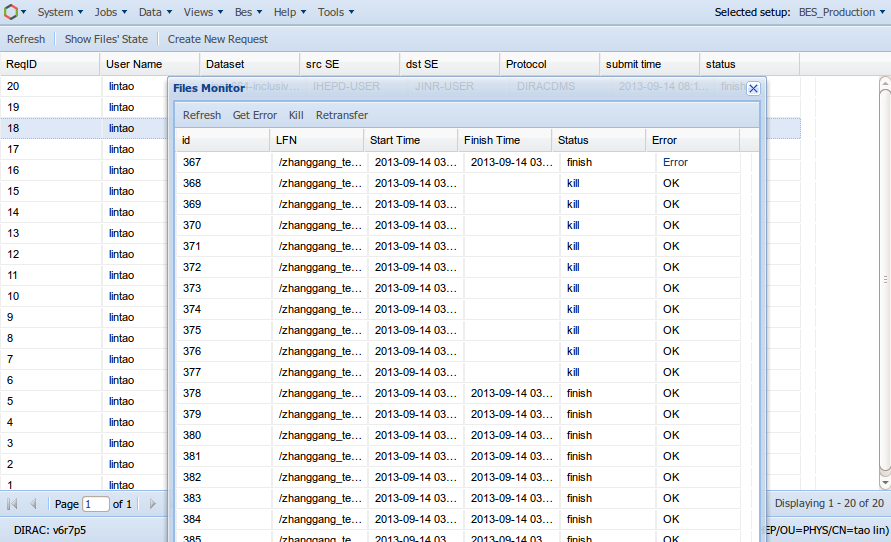
\includegraphics[width=\textwidth,keepaspectratio]{figures/transreqlist-with-kill-retransfer.png}
        \end{column}
        \begin{column}{.45\textwidth}
            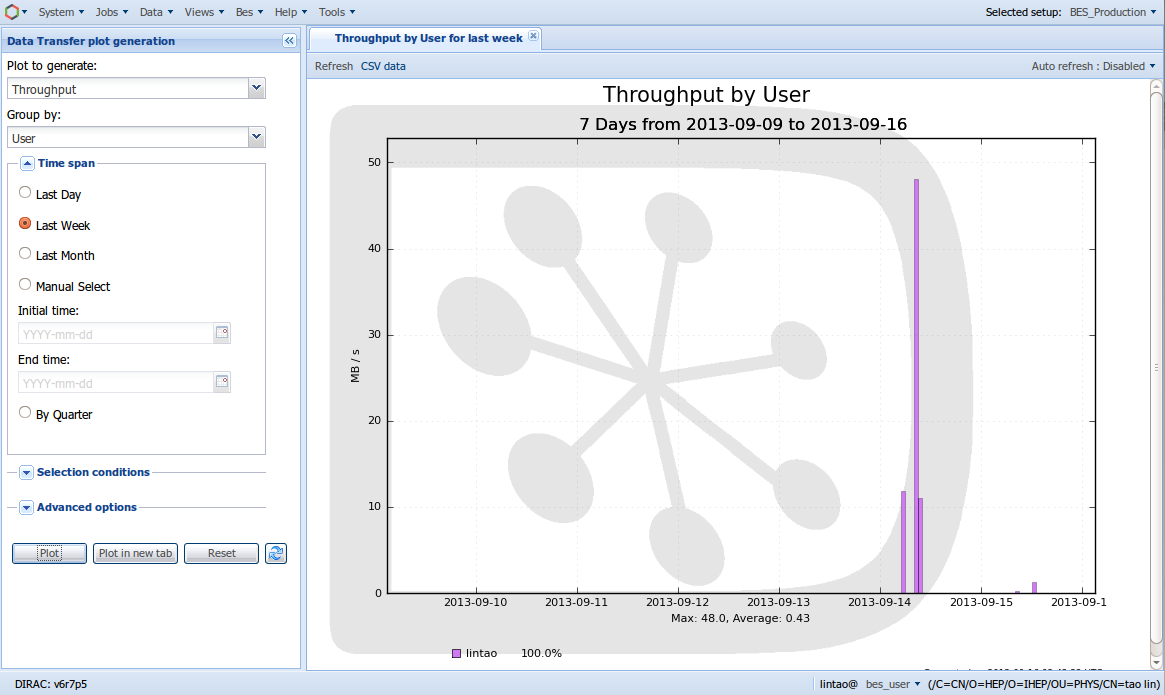
\includegraphics[width=\textwidth,keepaspectratio]{figures/acct-throughput-last-week.png}
        \end{column}
    \end{columns}
\end{myblock}

\begin{myblock}{Conclusion and Outlook}
    \begin{itemize}
        \item Conclusion 
            \begin{itemize}
            \item The design and implementation of BESDIRAC Tranfser System 
                  was presented.
            \item The building of the prototype system makes us earn the 
                  experience to deal with DIRAC.
            \item DIRAC is flexible to extend its functionality.
            \item Users can use both command line tools and web portal
                  to submit and monitor transfer requests.
            \end{itemize}
        \item Outlook
            \begin{itemize}
            \item Work on BESDIRAC Transfer system is ongoing.
            %\item 
            %\item The User Access Control should be implemented.
            \end{itemize}
    \end{itemize}
\end{myblock}

            \end{beamercolorbox}
        \end{column}
        % --------------------------------------------------------------------
        \begin{column}{.01\textwidth}
        \end{column}
        % --------------------------------------------------------------------
    \end{columns}
\end{frame}
\end{document}

